\section{Comparison to Differential Causal Effect}\label{sec:DCE}

This appendix details the Differential Causal Effect comparison summarised in \cref{sec:evaluation}.

Having tested \ourapproach against ground truth in
\cref{sub:synthetic}, we now compare it with gradient-based
attribution on a continuous-input credit-limit example.

A natural baseline for continuous-input attribution is to read causal influence off
the gradient of an interventional mean function. The motivation is direct:
$\mathbb{E}\!\bigl[Y\mid do(X{=}1)\bigr]-\mathbb{E}\!\bigl[Y\mid do(X{=}0)\bigr]$
is the binary ATE, and for a continuous cause one ``arrives at derivative
calculus'' \citep[Section~7.4.3]{ness2025causal} by letting the contrast shrink:
$\partial_x\,\mathbb{E}\!\bigl[Y\mid do(X{=}x)\bigr]$. Generalised to a vector
$\mathbf{x}=(x_1,\ldots,x_d)$ with interventional mean
$m(\mathbf{x})=\mathbb{E}\!\bigl[Y_{\mathbf{X}=\mathbf{x}}\bigr]$, the
\emph{causal gradient} is
\[
\nabla_{\mathbf{x}}\,m(\mathbf{x})
=\Bigl(\partial_{x_1}\mathbb{E}\!\bigl[Y_{\mathbf{X}=\mathbf{x}}\bigr],\;\ldots,\;
        \partial_{x_d}\mathbb{E}\!\bigl[Y_{\mathbf{X}=\mathbf{x}}\bigr]\Bigr),
\]
and each partial is the \emph{differential causal effect} (DCE) of a single
variable at $\mathbf{x}$. \citet{butler2022differential} introduced this
quantity in the Gaussian Process regression setting, where, with the posterior
expected mean expressible as $\sum_n k(x,x^{(n)})\alpha_n$, the DCE has the
closed form $\partial_{x_i}\hat{F}=\sum_n \partial_{x_i}k(x,x^{(n)})\alpha_n$.

\ourapproach and DCE are not direct competitors (DCE estimates a rate of
change, \ourapproach estimates individual-level responsibility), but
\ourapproach inherits the territory of continuous attribution, so a contrast
on a single example is informative. We highlight the differences:
\begin{enumerate}
\item DCE requires $y=F(\mathbf{X},\epsilon)$ with $F$ differentiable;
  \ourapproach requires only that the causal model be sampleable, and the
  inference algorithm for the expanded model is the user's choice (we use Monte
  Carlo throughout).
\item DCE inherits the units of both $\mathbf{X}$ and $Y$, so cross-feature
  comparison is unit-sensitive. The \ourapproach score integrates over the
  necessity- and sufficiency-world densities, so changes to input scale leave
  the score essentially unchanged.\footnote{This unit-invariance is contingent
  on how the alternative-value distribution $\Delta$ is specified. The
  $\epsilon$-excised $\Delta$ of Section~\ref{sec:causal_impact} is invariant to
  a reparameterisation of the input scale precisely when $\epsilon$ is fixed by
  the \emph{probability mass} excised around the factual value (equivalently, in
  standardised units), as in the ROPE/effect-size reading given there, rather
  than as an absolute distance in the raw units of $\mathbf{X}$: an
  absolute-distance $\epsilon$ held fixed across a rescaling would itself become
  unit-dependent and reintroduce the very sensitivity PCI otherwise avoids.}
\item DCE varies abruptly with the local geometry of $F$. The \ourapproach
  score depends on where the factual value sits relative to the
  necessity/sufficiency densities and is therefore non-zero in flat regions
  while remaining locally informative.
\end{enumerate}

\begin{example}[credit-limit assignment]\label{ex:age}
We model an applicant's approved credit limit as a function of \emph{age} and
the \emph{time of application}. The deterministic component is a sigmoidal
rise in age with a small sinusoidal modulation in time-of-day; intuitively,
age should dominate. We consider four settings on two axes: time measured in
hours vs.\ minutes (a units rescaling that should not affect attribution), and
an age prior centred at $30$ vs.\ $40$ (a genuine change in what counts as
unusual). The deterministic component is shown in
Figure~\ref{fig:internal}. Computational details and code are in
\texttt{docs/source/gradient\_based\_attribution.ipynb}.
\end{example}

\begin{figure}[t]
    \centering
    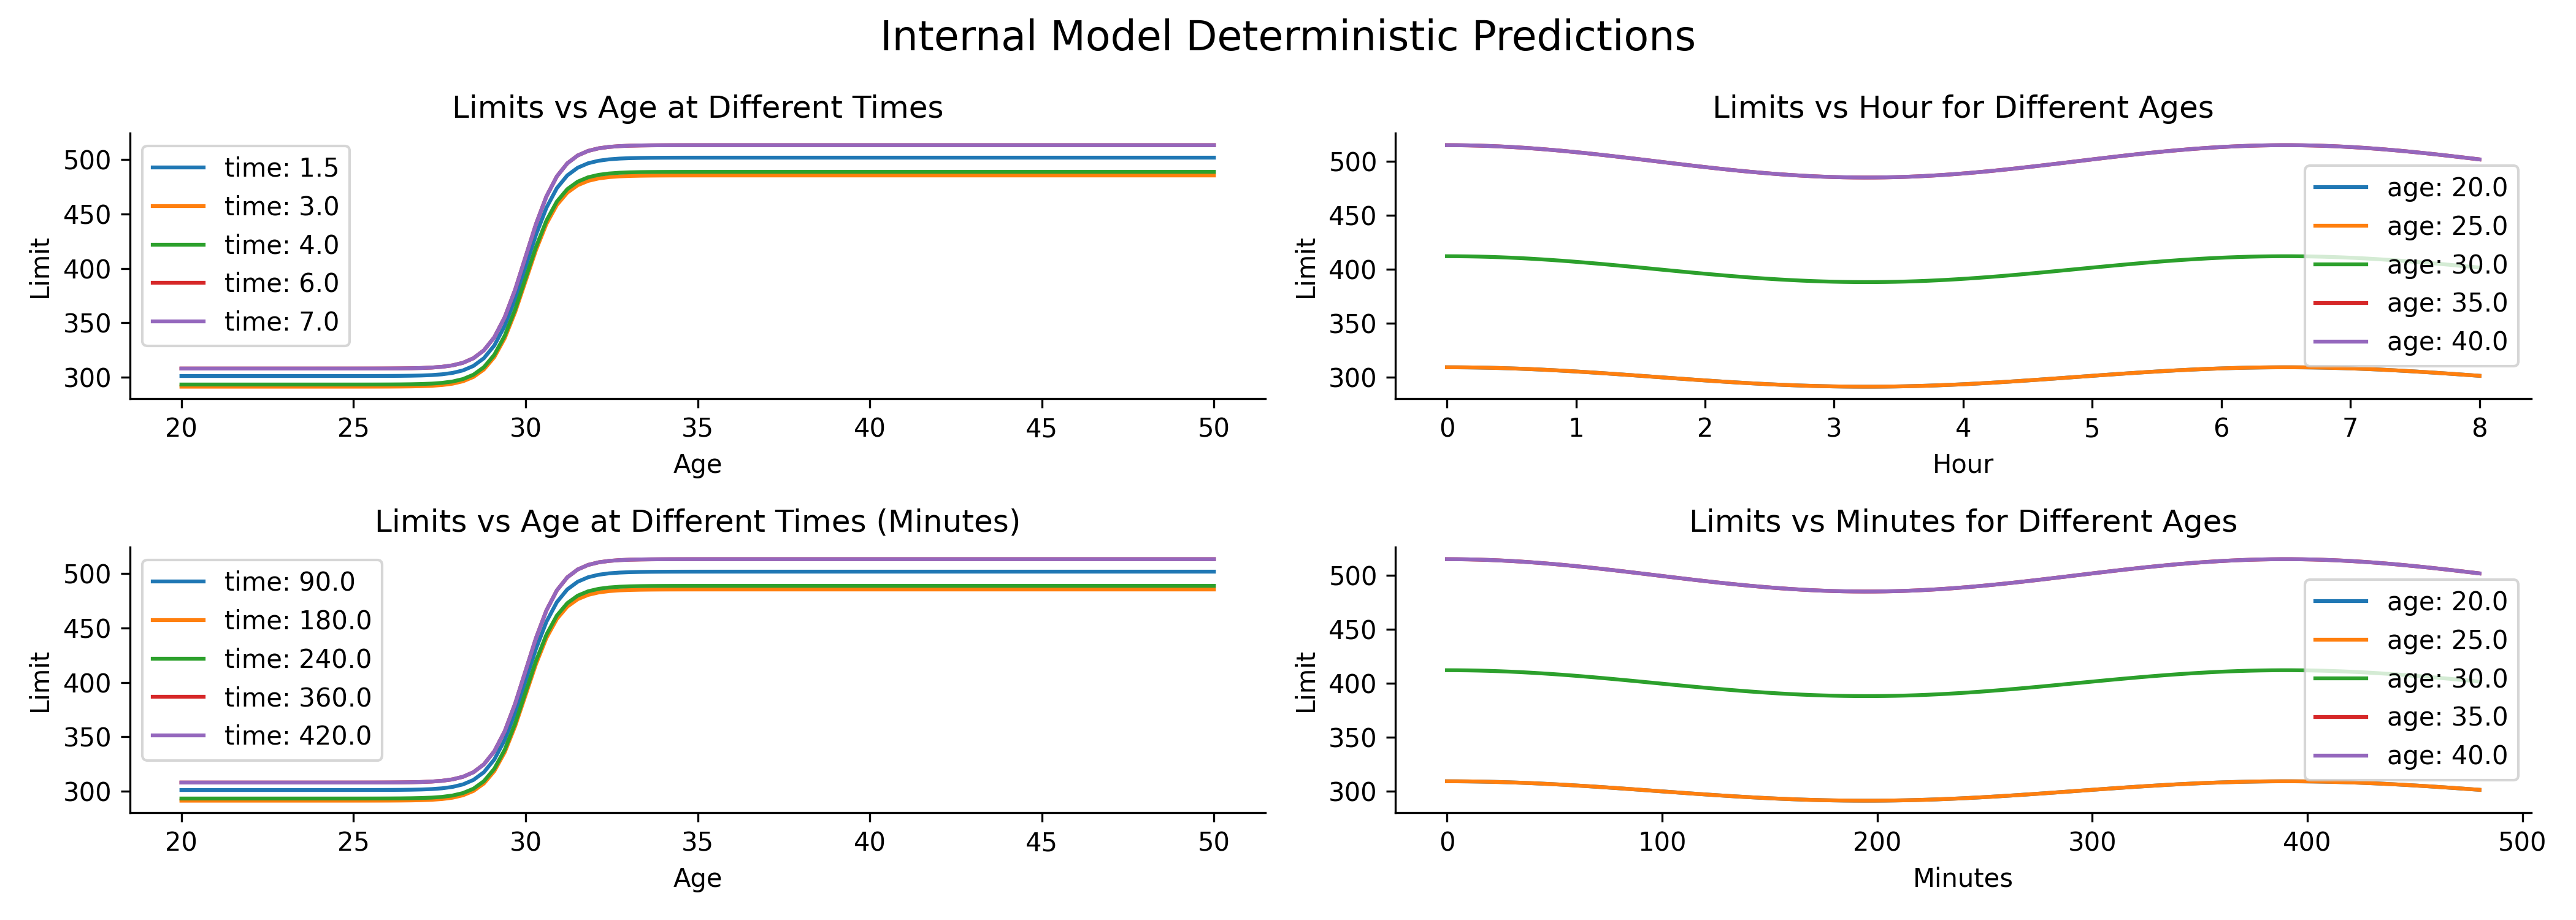
\includegraphics[width=\linewidth]{figures/internal_model_predictions.png}
    \caption{Deterministic component of the credit-limit model
    (Example~\ref{ex:age}), on the hours scale: limit vs.\ age at several times
    of day (left) and limit vs.\ time of day at several ages (right). Age
    dominates the limit, with a small sinusoidal modulation from time of day;
    the minute scale is identical modulo a linear reparameterisation (verified
    in the notebook).}\label{fig:internal}
\end{figure}

\paragraph{\ourapproach scores.} We instantiate $ci$ as the absolute-difference
score from Example~\ref{ex:absolute_score}, $ci(y^s,y^n,y^\star)=|y^n-y^\star|-|y^s-y^\star|$,
and run the search of Section~\ref{sec:causal_impact} on each setting,
conditioning on age and on time of application as singleton suspects.
Figure~\ref{fig:mechanism} shows the mechanism for the canonical setting
(age-$30$ prior, hours): when age is the active suspect the necessity-world
outcome tracks the deterministic curve while the sufficiency-world outcome
stays near factual, and the same picture, with a smaller displacement, holds
for time of application. Table~\ref{tab:dce_means} reports the mean total
scores across all four settings. Two patterns stand out. First, age outscores
time of application in every setting, by roughly a factor of $3/2$, matching the
intuition that the age sigmoid moves the outcome by a much larger absolute
amount than the daily modulation does. Second, the scores are essentially
unchanged between the hours and minutes columns, confirming the unit-invariance
discussed above, whereas the shift from the age-$30$ to the age-$40$ prior
raises every score, since a more unusual factual age means a larger search-space
displacement.

\begin{figure}[t]
    \centering
    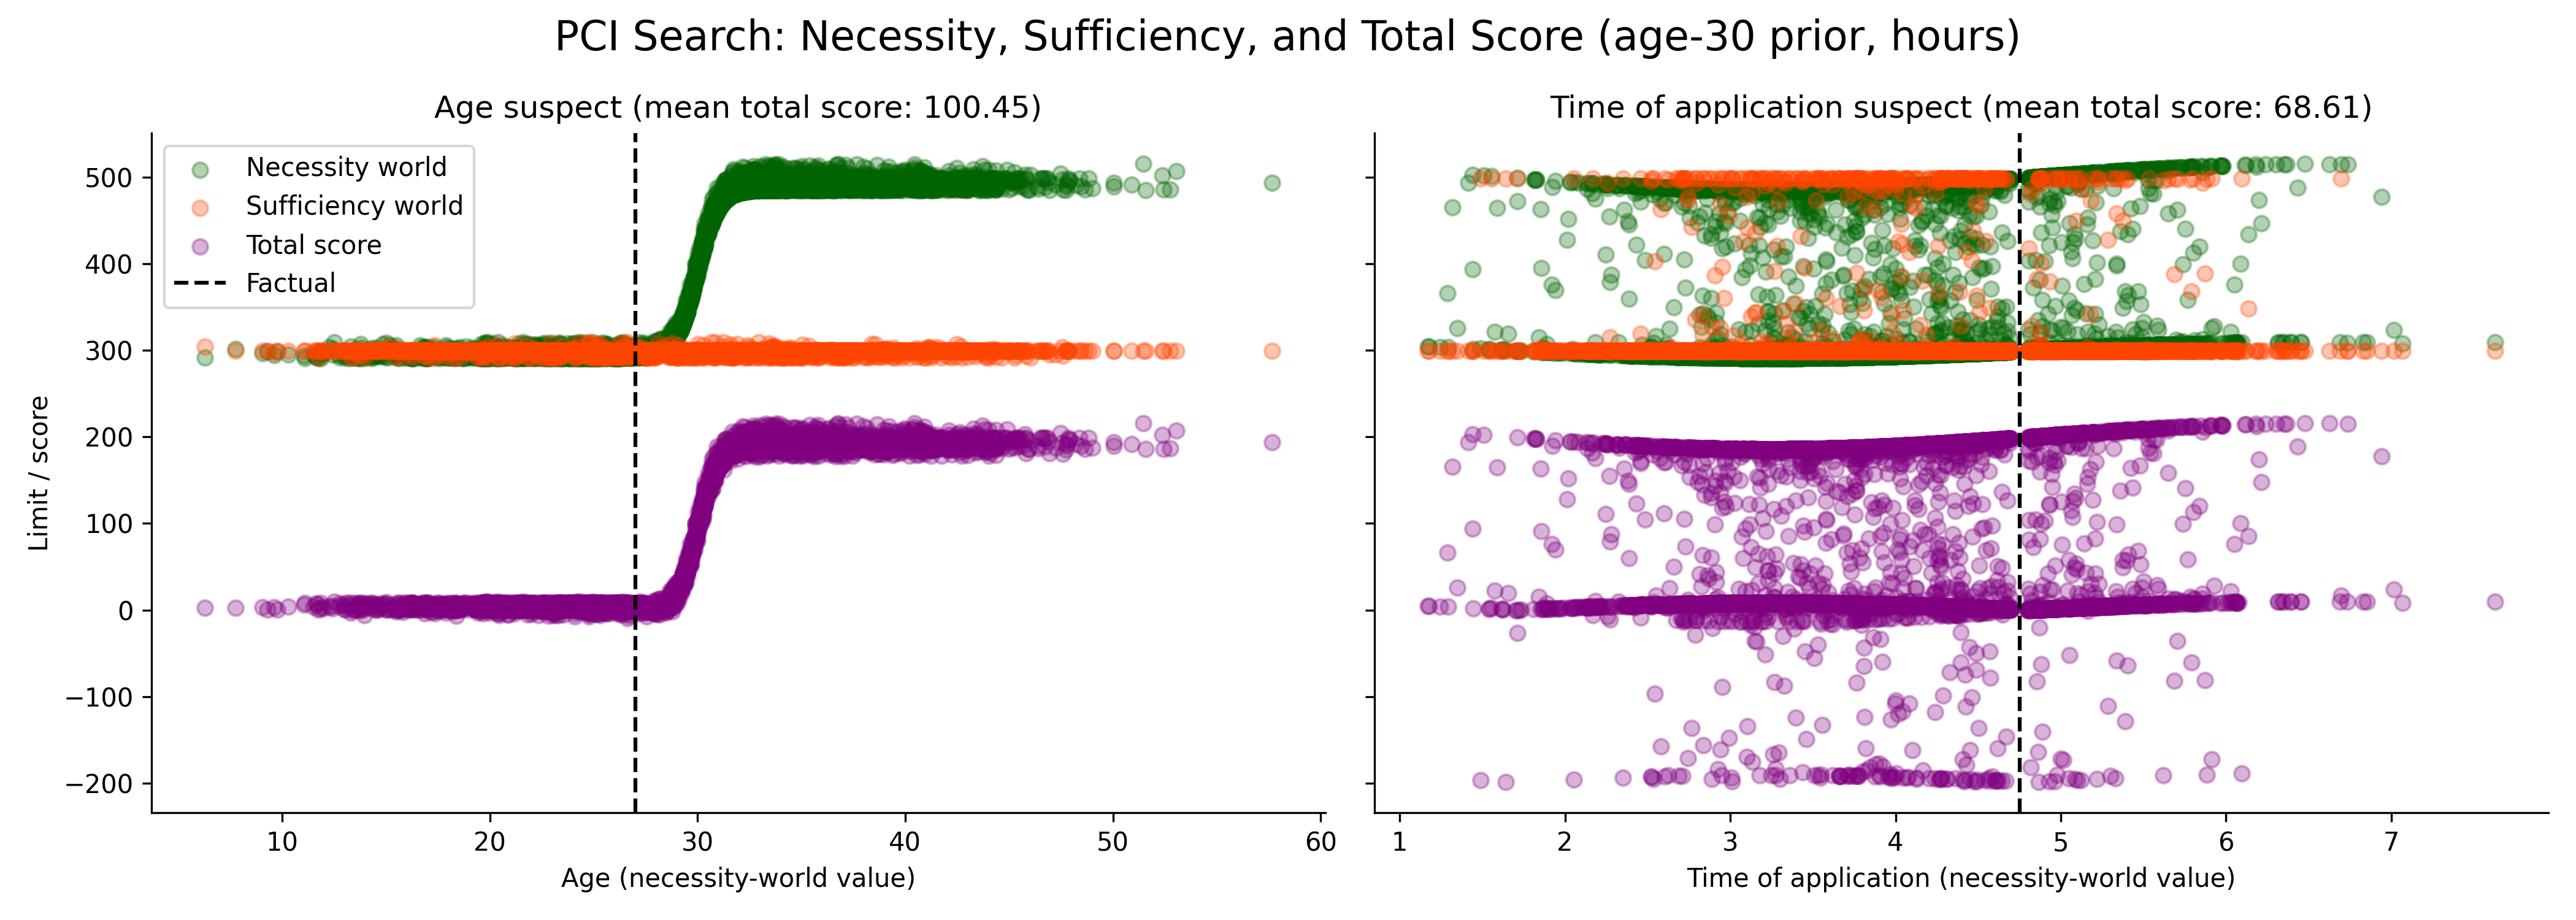
\includegraphics[width=\linewidth]{figures/search_samples_combined.png}
    \caption{PCI search for the canonical setting (age-$30$ prior, hours), with
    age (left) and time of application (right) as the active suspect.
    Necessity-world (green) and sufficiency-world (orange) limit samples and the
    total score (purple) are plotted against the necessity-world value of the
    suspect; the dashed line marks the factual. The necessity world departs from
    factual along the deterministic response while the sufficiency world stays
    near it; each panel title gives the mean total score.}\label{fig:mechanism}
\end{figure}

\begin{table}[t]
\centering
\caption{Mean \ourapproach total scores for age and time of application across
the four settings (time unit $\times$ age prior), at the factual instance. Age
outscores time in every setting; the hours and minutes columns agree
(unit-invariance), while the age-$40$ prior raises all scores relative to
age-$30$ (a more unusual factual age).}
\label{tab:dce_means}
\vspace{4pt}
\begin{tabular}{l cc cc}
\toprule
& \multicolumn{2}{c}{age-$30$ prior} & \multicolumn{2}{c}{age-$40$ prior} \\
\cmidrule(lr){2-3}\cmidrule(lr){4-5}
Suspect & hours & minutes & hours & minutes \\
\midrule
Age                  & $100.45$ & $97.95$  & $177.87$ & $176.56$ \\
Time of application  & $68.61$  & $66.51$  & $117.97$ & $118.42$ \\
\bottomrule
\end{tabular}
\end{table}

\paragraph{PCI vs.\ DCE across the input grid.}
Figure~\ref{fig:contrast} contrasts the two methods on the same grid of factual
values (age-$30$ prior, hours); the other three settings give qualitatively the
same picture. The top panel plots the difference between the \ourapproach scores
for age and for time of application: it is positive everywhere, so age is
consistently the more responsible variable, with the gap largest near the steep
region of the age-limit sigmoid and growing for ages further from the prior
mean. The bottom panels show the DCE for the two inputs, and two differences
with \ourapproach stand out. First, on the hour scale the DCE for time of
application exceeds the DCE for age over most of the grid and traces a visible
sine wave, whereas \ourapproach reports age as the more responsible variable
everywhere. Second, switching the time unit from hours to minutes flattens the
time DCE by roughly a factor of $60$, making the unit sensitivity explicit. Both
are direct consequences of DCE's role as a rate-of-change estimator rather than
a responsibility score, and both make it harder to compare across features and
across reparameterisations.

\begin{figure}[t]
    \centering
    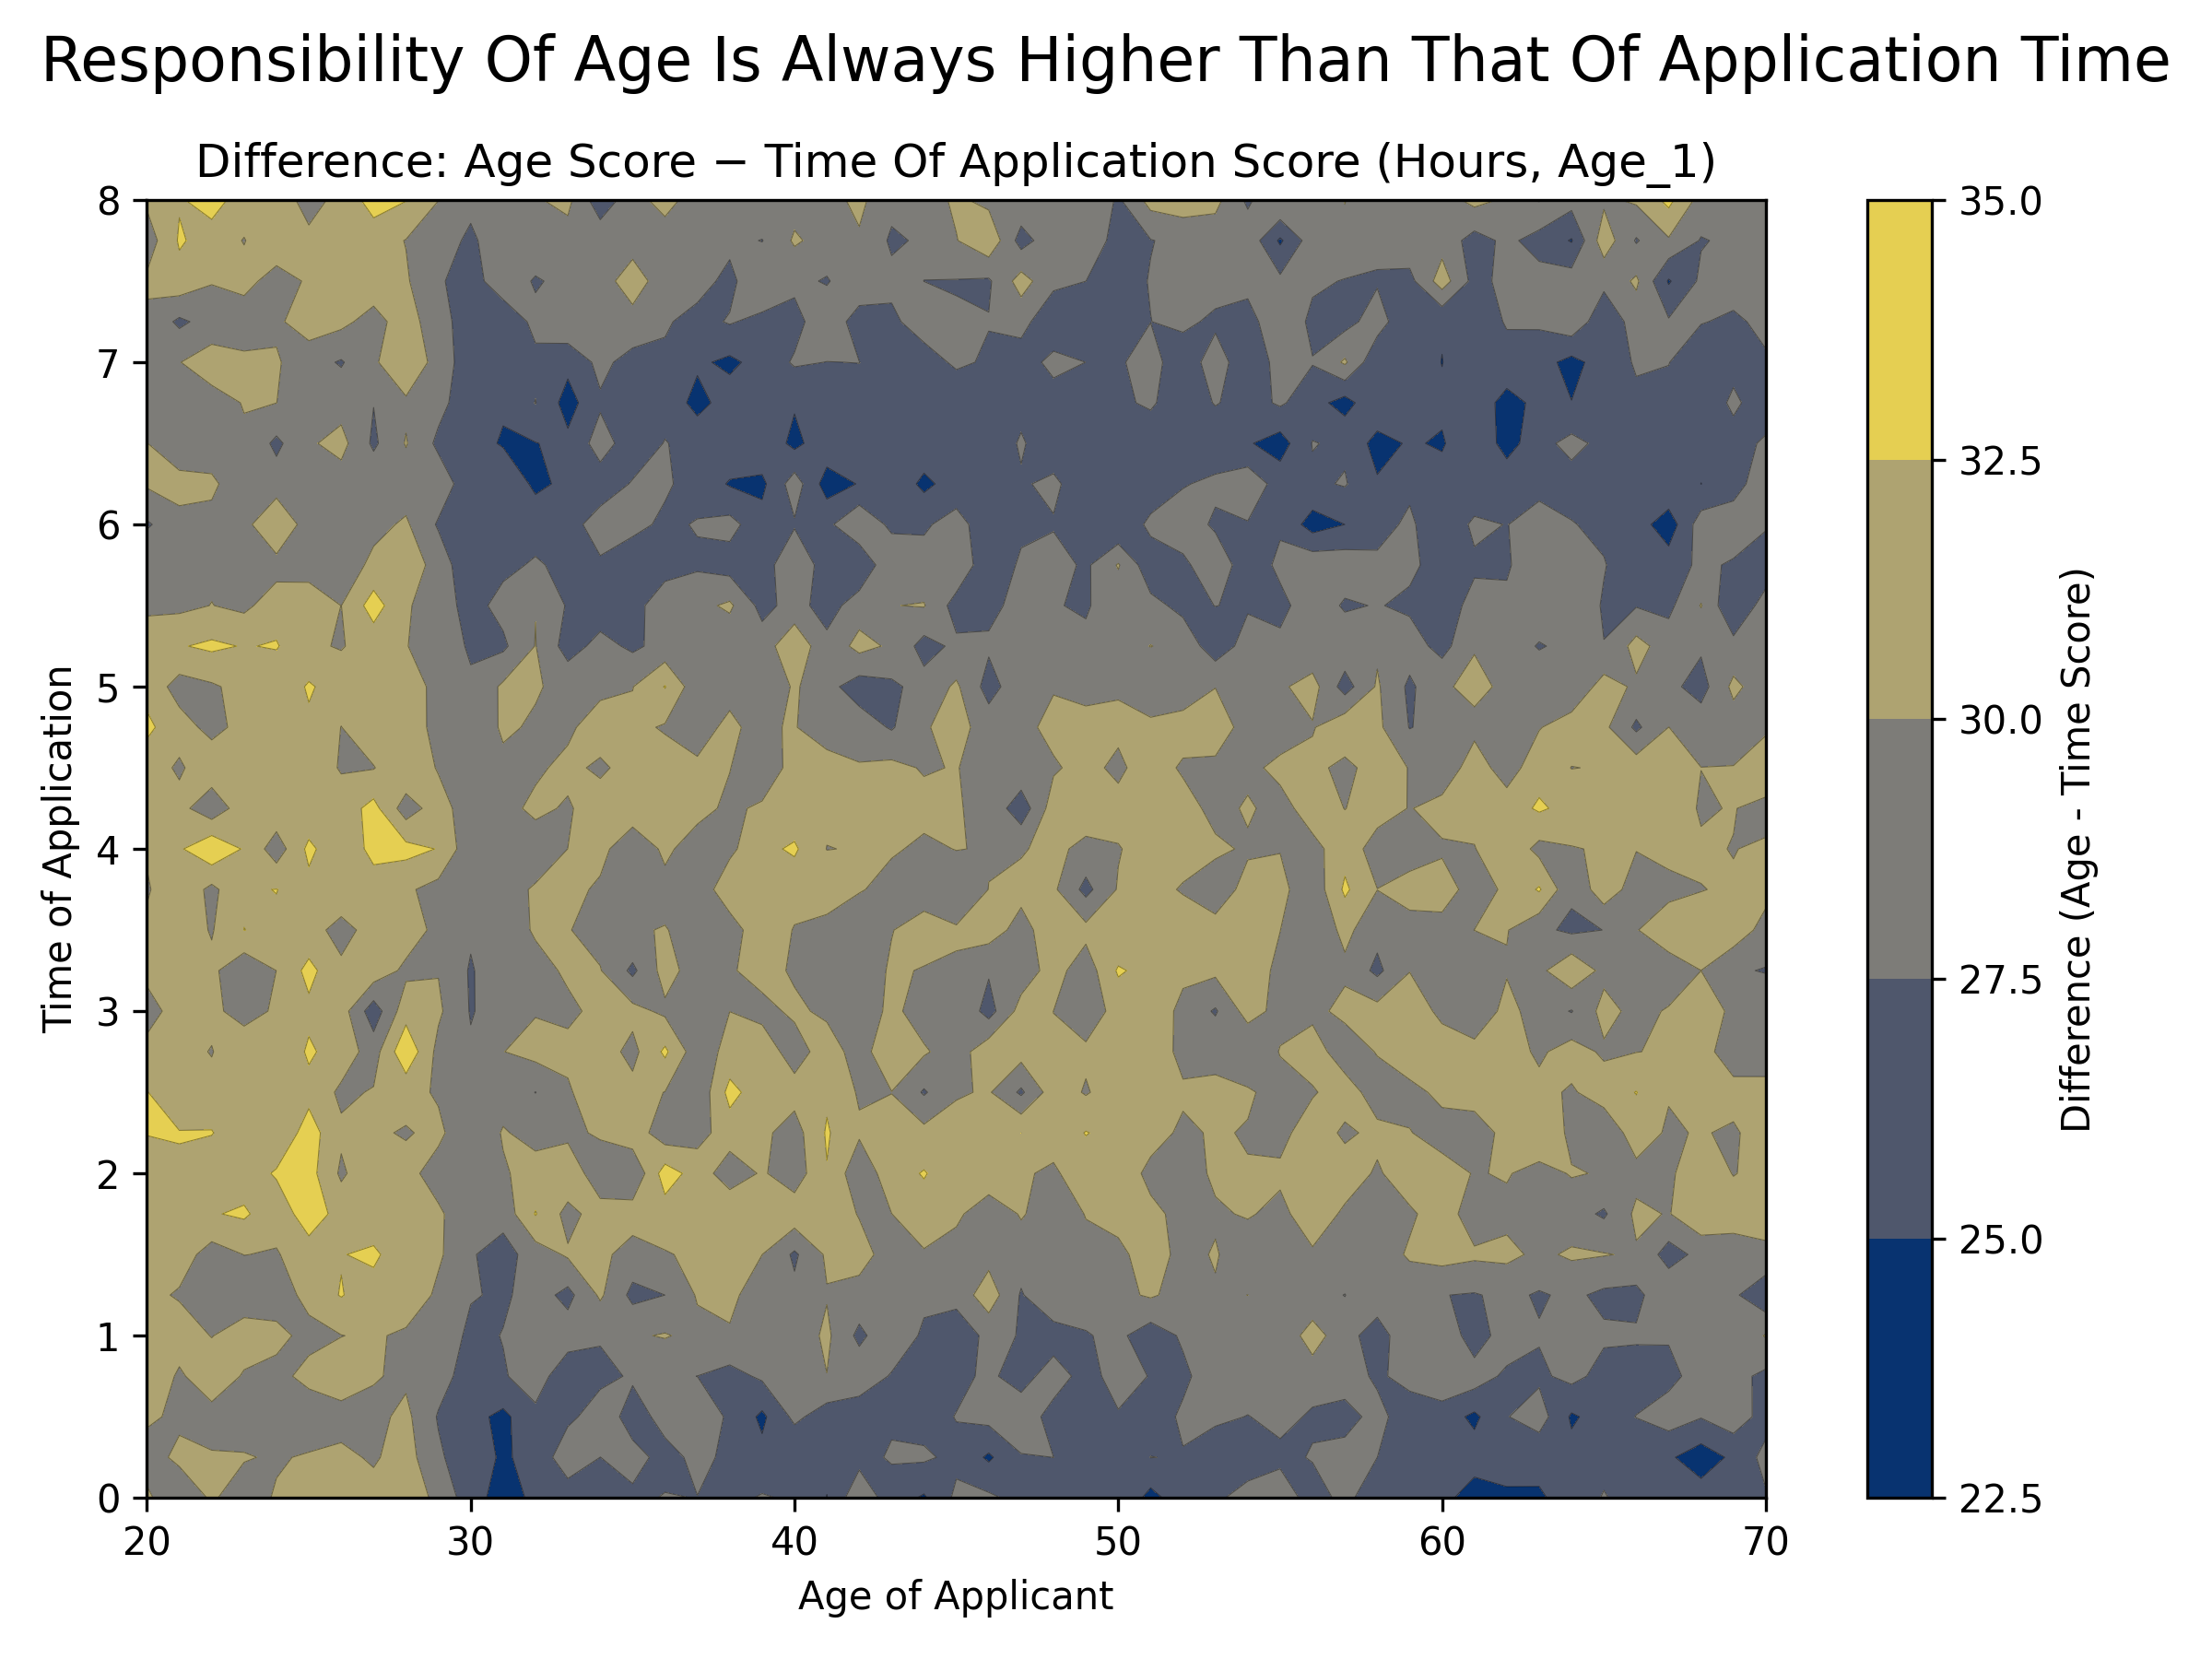
\includegraphics[width=0.62\linewidth]{figures/contour_diff_hours_age_1.png}\\[6pt]
    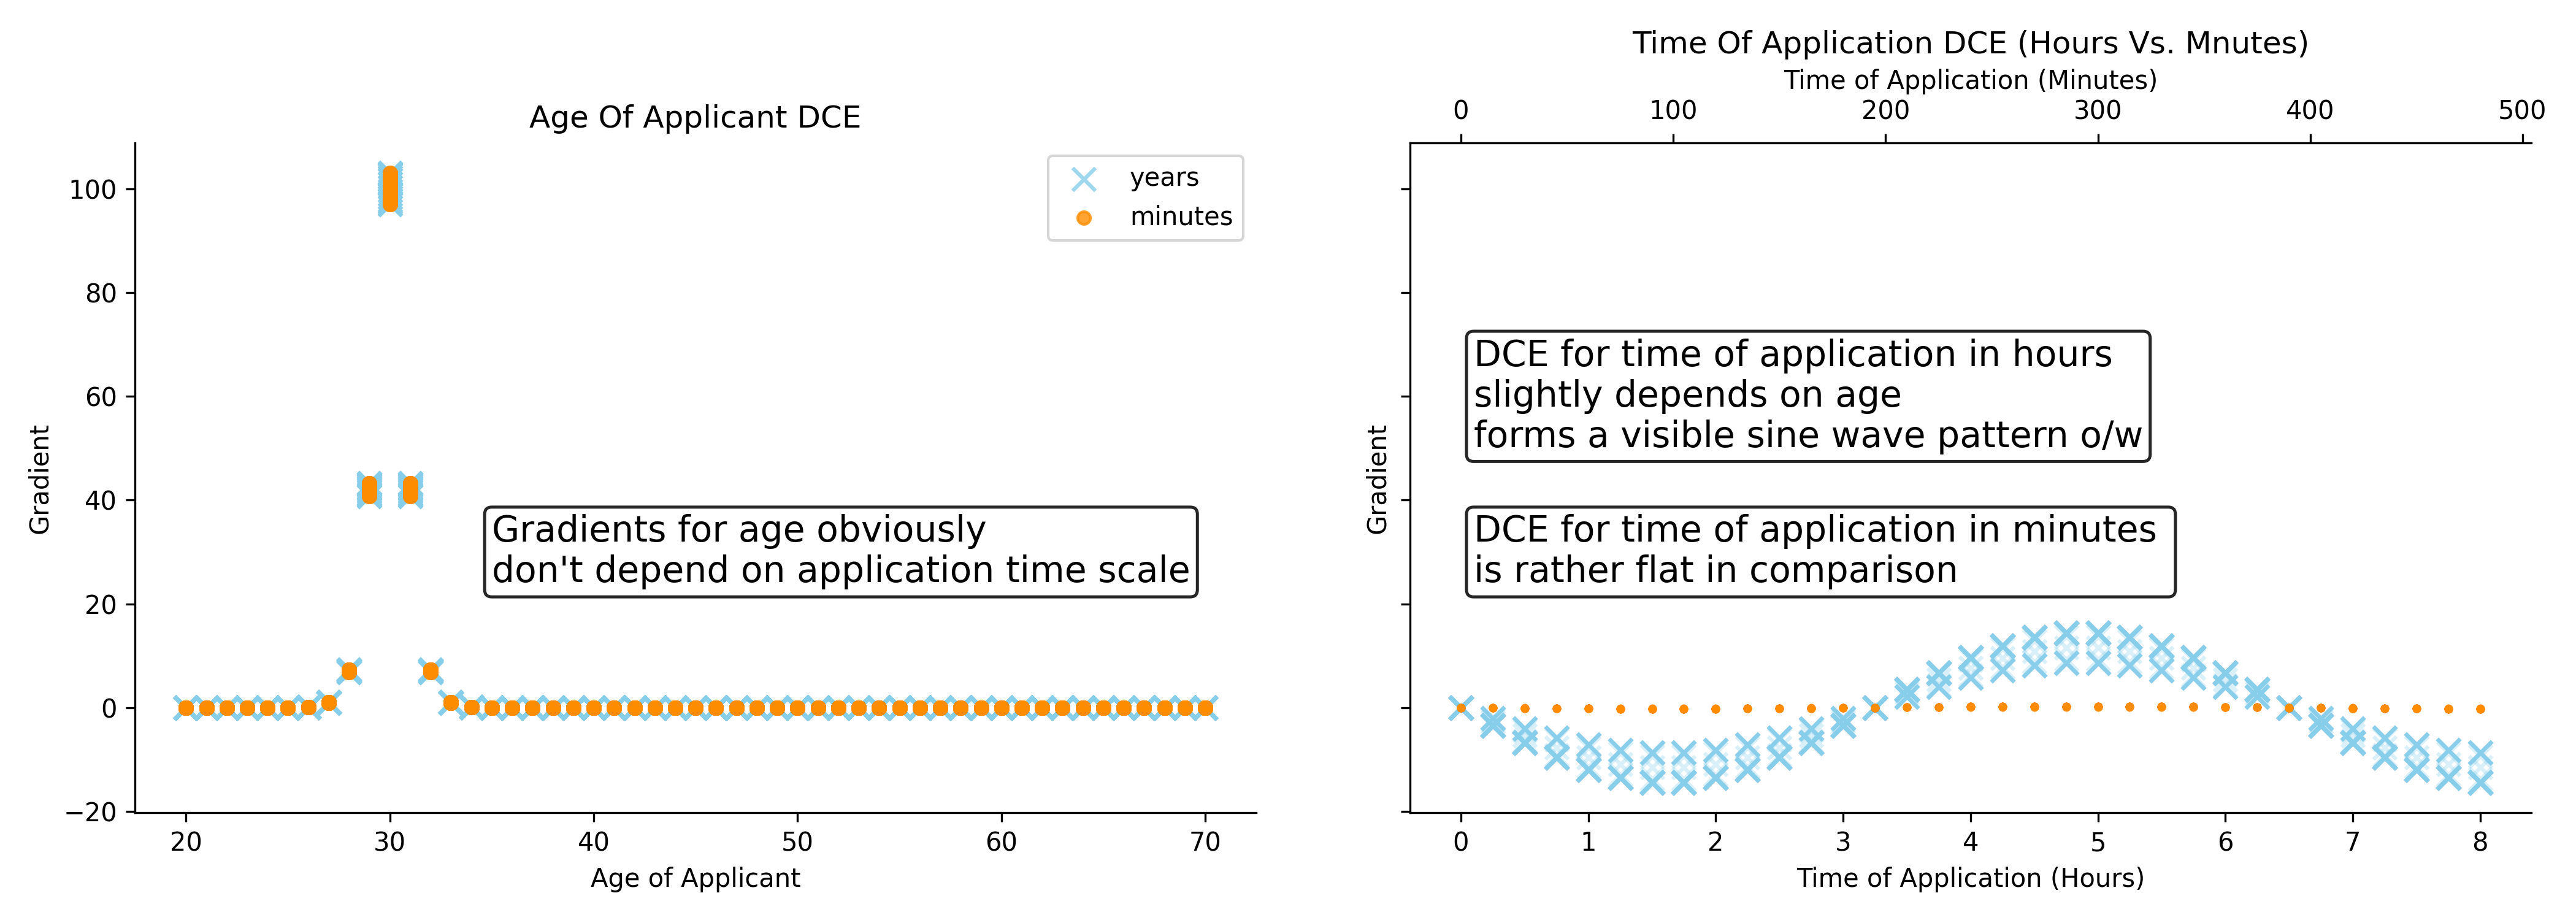
\includegraphics[width=\linewidth]{figures/dce_age_time_hours_minutes.png}
    \caption{\textbf{PCI vs.\ DCE on the credit-limit grid} (age-$30$ prior,
    hours). \emph{Top:} difference between the \ourapproach scores for age and
    for time of application; positive everywhere, largest near the steep region
    of the age-limit sigmoid and for ages far from the prior mean, so age is
    always the more responsible variable. \emph{Bottom:} DCE for age (left) and
    time of application (right) on both unit scales. Age has the larger absolute
    DCE only inside the narrow steep region of the sigmoid; elsewhere time of
    application dominates on the hour scale and goes comparatively flat on the
    minute scale, illustrating DCE's shape and unit sensitivity.}
    \label{fig:contrast}
\end{figure}

\FloatBarrier  % keep the DCE figures within this appendix, not the next
